\documentclass{article}
\usepackage[paperwidth=8cm, paperheight=2cm, margin = 0cm, top=0.5cm]{geometry}
\usepackage{amsmath}


\usepackage{pgf}
\usepackage{tikz}


\usetikzlibrary{arrows,automata}

\tikzstyle{source}  = [draw,circle,fill=black,thick,inner sep=0mm,minimum size=2mm]

\renewcommand{\vec}[1]{\boldsymbol{#1}}

\begin{document}
\begin{center}
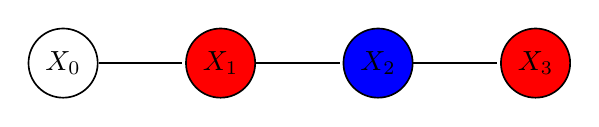
\begin{tikzpicture}[-,>=stealth',shorten >=1pt,auto,node distance=2cm,semithick]
                    
\node[state] (X1)               {$X_{0}$}; 
\node[state, fill=red] (X2) [right of=X1] {$X_{1}$};                   
\node[state, fill=blue] (X3) [right of=X2] {$X_{2}$};                   
\node[state, fill=red] (X4) [right of=X3] {$X_{3}$};    

\path
	(X1) edge (X2)
	(X2) edge (X3)
	(X3) edge (X4);
               
\end{tikzpicture}
\end{center}
\end{document}
